\documentclass[11pt,a4paper]{article}

\usepackage[utf8]{inputenc}
\usepackage[T1]{fontenc}
\usepackage[margin=1in]{geometry}
\usepackage{amsmath,amssymb,amsfonts}
\usepackage{graphicx}
\usepackage{xcolor}
\usepackage{booktabs}
\usepackage{tabularx}
\usepackage{array}
\usepackage{listings}
\usepackage{tikz}
\usetikzlibrary{shapes.geometric, arrows.meta, positioning, calc, fit}
\usepackage{enumitem}
\usepackage{caption}
\usepackage{subcaption}
\usepackage{float}
\usepackage{hyperref}

\hypersetup{
    colorlinks=true,
    linkcolor=black,
    citecolor=black,
    urlcolor=blue!70!black,
    pdftitle={DNS Hierarchy and Resolver},
    pdfauthor={Subham Bhat}
}

\definecolor{codebg}{rgb}{0.96,0.96,0.96}
\definecolor{codeframe}{rgb}{0.25,0.25,0.25}
\definecolor{codenum}{rgb}{0.45,0.45,0.45}

\lstset{
    backgroundcolor=\color{codebg},
    basicstyle=\ttfamily\footnotesize,
    breakatwhitespace=false,
    breaklines=true,
    captionpos=b,
    commentstyle=\color{codenum}\itshape,
    keywordstyle=\bfseries,
    numberstyle=\tiny\color{codenum},
    numbers=left,
    numbersep=8pt,
    frame=single,
    rulecolor=\color{codeframe},
    tabsize=4,
    columns=flexible,
    keepspaces=true,
    showspaces=false,
    showstringspaces=false,
    xleftmargin=14pt,
    xrightmargin=4pt,
    literate={→}{{$\rightarrow$}}1 {←}{{$\leftarrow$}}1 {–}{{--}}1 {—}{{---}}1 {·}{{$\cdot$}}1 {✓}{{OK}}2 {✗}{{X}}1
}

\newcolumntype{Y}{>{\raggedright\arraybackslash}X}

% screenshot from docs/screenshots (skipped quietly if the file is missing)
\newcommand{\shot}[3][0.92\textwidth]{%
  \IfFileExists{docs/screenshots/#2}{%
  \begin{figure}[H]\centering
  \includegraphics[width=#1,keepaspectratio]{docs/screenshots/#2}
  \caption{#3}\end{figure}}{}}

\emergencystretch=3em
\setlength{\parindent}{1.5em}
\setlength{\parskip}{0.4em}

\begin{document}

% ==============================================================================
% TITLE PAGE
% ==============================================================================
\begin{titlepage}
    \centering
    \vspace*{4.2cm}

    {\LARGE \textbf{The Domain Name System: A Four-Level}}\\[0.7em]
    {\LARGE \textbf{Naming Hierarchy, Recursive and Iterative}}\\[0.7em]
    {\LARGE \textbf{Resolution, Caching, and Cache Poisoning}}\\[1.4em]

    {\large for Computer Networks Laboratory}

    \vspace{3.8cm}

    {\large
    \textbf{Name:} Subham Bhat\\[0.55em]
    \textbf{Class:} BCSE III\\[0.55em]
    \textbf{Roll:} 002410501020\\[0.55em]
    \textbf{Group:} A1\\[0.55em]
    \textbf{College:} Jadavpur University
    }

    \vfill
    {\normalsize 1}
\end{titlepage}

% ==============================================================================
% TABLE OF CONTENTS
% ==============================================================================
\pagenumbering{roman}
\setcounter{page}{2}
\tableofcontents
\newpage

% ==============================================================================
% MAIN CONTENT
% ==============================================================================
\pagenumbering{arabic}
\setcounter{page}{3}

\section{Introduction}
\noindent People remember names; IP routes packets by address. The \textbf{Domain Name System} (\textbf{DNS}, RFC 1034 and RFC 1035) is the distributed database that maps one to the other. No single server could hold every name or answer every query, so the name space is a \textbf{tree} split into \textbf{zones}, each served by its own \textbf{authoritative} servers:
\begin{itemize}[leftmargin=2em]
    \item \textbf{Root servers} know only who serves each top-level domain.
    \item \textbf{TLD servers} (\texttt{.edu}, \texttt{.com}, \ldots) know who serves each second-level domain.
    \item \textbf{Authoritative servers} hold the actual records of their zone.
\end{itemize}
A client does not walk this tree itself. It sends one query to a \textbf{resolver}, which either walks the tree (\textbf{iterative} resolution, following referrals) or passes the question to a server that does it on its behalf (\textbf{recursive} resolution). Every answer carries a \textbf{TTL}, and resolvers \textbf{cache} answers, including ``no such name'' (RFC 2308), which is what keeps DNS fast. DNS normally runs over \textbf{UDP port 53}, falling back to TCP when an answer does not fit in 512 bytes.

\subsection{What Was Built}
This module builds a complete DNS laboratory in pure Java 11 with no external libraries:
\begin{enumerate}[leftmargin=2em]
    \item \textbf{RFC 1035 wire format:} encoding and decoding of all five message sections, name compression, and A, NS, CNAME, SOA, PTR, MX, TXT and AAAA records, with a byte-level dissector.
    \item \textbf{A four-level hierarchy of real authoritative servers}, each on its own loopback address: a lab root, \texttt{edu.}, \texttt{myuniv.edu.} and \texttt{cse.myuniv.edu.} (which holds the Assignment~6 records), loaded from BIND-style zone files.
    \item \textbf{Both resolution methods:} iterative and recursive, animated side by side message by message.
    \item \textbf{A caching resolver} on port 53 (and 5300) that Windows \texttt{nslookup} can use, with TTL countdown, negative caching, bailiwick checks on glue, and detection of transparent DNS interception.
    \item \textbf{UDP truncation} (TC=1) and \textbf{TCP fallback} for large answers.
    \item \textbf{A cache-poisoning experiment:} 65,536 forged replies against a 2008-style resolver and against a modern one.
    \item \textbf{A live dashboard} on \texttt{http://localhost:8084}.
\end{enumerate}

\begin{table}[H]
\centering
\caption{The lab name servers}
\small
\begin{tabularx}{\textwidth}{@{}llY@{}}
\toprule
\textbf{Address} & \textbf{Server name} & \textbf{Zone} \\ \midrule
127.0.0.10 & \texttt{a.root-servers.lab} & \texttt{.} (lab root): delegates \texttt{edu.} and the reverse zone \\
127.0.0.11 & \texttt{ns.edu-servers.lab} & \texttt{edu.}: delegates \texttt{myuniv.edu.} \\
127.0.0.12 & \texttt{ns1.myuniv.edu} & \texttt{myuniv.edu.}: delegates \texttt{cse.myuniv.edu.} \\
127.0.0.13 & \texttt{dns.cse.myuniv.edu} & \texttt{cse.myuniv.edu.}: \texttt{www} = 192.168.151.4, \texttt{web} (CNAME), MX, \ldots \\
127.0.0.1:53 / :5300 & resolver & Caching recursive resolver for clients \\ \bottomrule
\end{tabularx}
\end{table}

\shot{02_tree_walk.png}{Walking the tree with an empty cache: root, \texttt{edu}, \texttt{myuniv}, \texttt{cse}.}

% ==============================================================================
\section{The RFC 1035 Message Format}
Queries and responses share one format: a fixed 12-byte header followed by four variable sections.

\begin{figure}[H]
\centering
\begin{lstlisting}[numbers=none, frame=none, backgroundcolor=\color{white}, basicstyle=\ttfamily\footnotesize]
+----------------+----------------------------------------------------+
|  ID (16 bits)  | QR | Opcode | AA | TC | RD | RA | Z | RCODE         |
+----------------+----------------------------------------------------+
|  QDCOUNT       |  ANCOUNT       |  NSCOUNT       |  ARCOUNT          |
+----------------+----------------------------------------------------+
|  Question:   QNAME  QTYPE  QCLASS                                    |
|  Answer:     resource records  (NAME TYPE CLASS TTL RDLENGTH RDATA)  |
|  Authority:  NS records of the zone that should be asked next        |
|  Additional: glue (A records of those name servers), ...             |
+---------------------------------------------------------------------+
\end{lstlisting}
\caption{DNS message layout: 12-byte header and four sections.}
\end{figure}

\begin{table}[H]
\centering
\caption{Header flags used in this lab}
\small
\begin{tabularx}{\textwidth}{@{}lY@{}}
\toprule
\textbf{Flag} & \textbf{Meaning} \\ \midrule
QR & 0 = query, 1 = response. \\
AA & Authoritative Answer: the responding server owns the zone. \\
TC & Truncated: the answer did not fit in a 512-byte UDP datagram; retry over TCP. \\
RD & Recursion Desired: set by the client to ask the server to find the final answer. \\
RA & Recursion Available: set by a server that is willing to recurse. \\
RCODE & 0 NOERROR, 2 SERVFAIL, 3 NXDOMAIN, 5 REFUSED. \\ \bottomrule
\end{tabularx}
\end{table}

\textbf{Name compression.} A name is a sequence of length-prefixed labels ending in a zero byte: \texttt{www.cse.myuniv.edu} is \texttt{03 www 03 cse 06 myuniv 03 edu 00}. Because the same suffix appears many times in a response, any suffix that occurred earlier is replaced by a 2-byte \textbf{pointer} whose top two bits are \texttt{11}: \texttt{C0 0C} means ``the rest of this name is at offset 12'', which is where the question name starts, right after the header.

\begin{lstlisting}[language=Java, caption={Encoding a name with compression pointers (\texttt{wire/Message.java}).}]
void name(String n, boolean compress) {
    String rest = n;
    while (!rest.isEmpty()) {
        Integer p = compress ? ptr.get(rest.toLowerCase()) : null;
        if (p != null) { u16(0xC000 | p); return; }               // pointer to an earlier copy
        if (pos() < 0x3FFF) ptr.putIfAbsent(rest.toLowerCase(), pos());
        int dot = rest.indexOf('.');
        String label = dot < 0 ? rest : rest.substring(0, dot);
        byte[] b = label.getBytes(StandardCharsets.US_ASCII);
        if (b.length > 63) throw new IllegalArgumentException("label longer than 63 bytes: " + label);
        u8(b.length); out.write(b, 0, b.length);                   // length-prefixed label
        rest = dot < 0 ? "" : rest.substring(dot + 1);
    }
    u8(0);                                                          // root label
}
\end{lstlisting}

\shot[0.88\textwidth]{04_packet_dissection.png}{The byte-level dissector: every field of a real response, including the \texttt{C0 0C} compression pointer.}

% ==============================================================================
\section{System Architecture}

\begin{figure}[H]
\centering
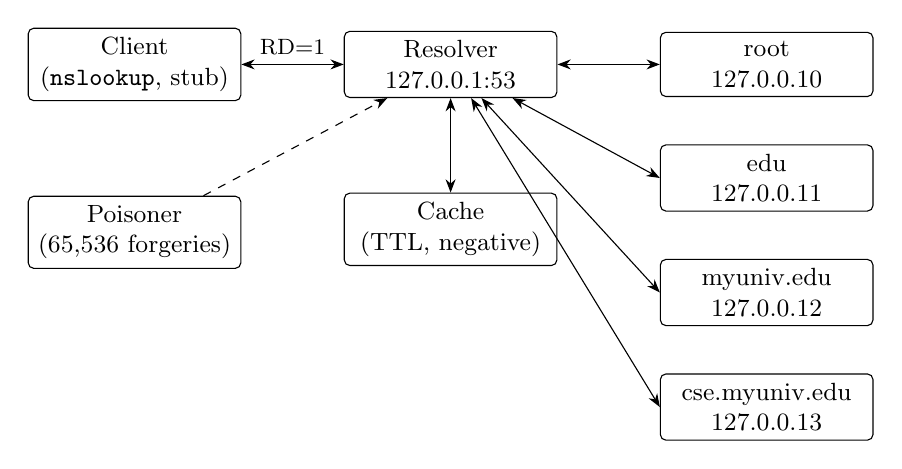
\begin{tikzpicture}[node distance=0.6cm, box/.style={draw, rounded corners=2pt, minimum width=2.7cm, minimum height=0.8cm, align=center, font=\small}, >=Stealth]
\node[box] (pc) {Client\\(\texttt{nslookup}, stub)};
\node[box, right=1.3cm of pc] (res) {Resolver\\127.0.0.1:53};
\node[box, right=1.3cm of res] (root) {root\\127.0.0.10};
\node[box, below=of root] (edu) {edu\\127.0.0.11};
\node[box, below=of edu] (my) {myuniv.edu\\127.0.0.12};
\node[box, below=of my] (cse) {cse.myuniv.edu\\127.0.0.13};
\node[box, below=1.2cm of res] (cache) {Cache\\(TTL, negative)};
\node[box, below=1.2cm of pc] (att) {Poisoner\\(65,536 forgeries)};
\draw[<->] (pc) -- node[above, font=\footnotesize]{RD=1} (res);
\draw[<->] (res) -- (root); \draw[<->] (res) -- (edu.west); \draw[<->] (res) -- (my.west); \draw[<->] (res) -- (cse.west);
\draw[<->] (res) -- (cache);
\draw[->, dashed] (att) -- (res);
\end{tikzpicture}
\caption{Components of the DNS module (iterative mode: the resolver asks every level itself).}
\end{figure}

\begin{table}[H]
\centering
\caption{Source packages}
\small
\begin{tabularx}{\textwidth}{@{}lY@{}}
\toprule
\textbf{Package} & \textbf{Responsibility} \\ \midrule
\texttt{wire/} & RFC 1035 encoder and decoder; records every field's byte span for the dissector. \\
\texttt{zone/} & BIND-style zone files: SOA, NS, A, CNAME, MX, PTR, TXT, AAAA. \\
\texttt{server/AuthServer} & Authoritative answers, referrals with glue, NXDOMAIN/NODATA with SOA, REFUSED, TC=1, and optional recursion. \\
\texttt{server/Listener} & UDP and TCP listeners (512-byte UDP limit, 2-byte length prefix on TCP). \\
\texttt{server/Resolver}, \texttt{Cache} & Iterative walk from root hints, bailiwick check, CNAME chasing, TTL and negative cache, secure upstream queries. \\
\texttt{attack/Poisoner} & The Kaminsky-style forgery race. \\
\texttt{client/DnsClient} & Stub client used by the tests and the dashboard. \\ \bottomrule
\end{tabularx}
\end{table}

% ==============================================================================
\section{Implementation and Workflows}

\subsection{Authoritative Servers}
Each lab server answers from its own zones only. For a name in its zone it gives an authoritative answer (AA=1) and chases CNAMEs inside the zone, so \texttt{web.cse.myuniv.edu} returns the CNAME and the A record of \texttt{www}. For a name below a delegation it returns a \textbf{referral}: the NS records of the child zone in the Authority section and their A records as \textbf{glue} in the Additional section. A missing name gets NXDOMAIN and a missing type gets NODATA; both include the SOA so that resolvers can cache the negative answer. Names outside every zone get REFUSED. A UDP answer longer than 512 bytes is truncated with TC=1, and the client repeats the query over TCP.

\subsection{Iterative Resolution}
The resolver starts from the root hints, sends RD=0 queries, and follows each referral one level down. It accepts glue only if it lies inside the zone being delegated (the \emph{bailiwick check}); otherwise a malicious server could inject addresses for unrelated names.

\begin{table}[H]
\centering
\caption{Iterative lookup of \texttt{www.cse.myuniv.edu A} with an empty cache (measured)}
\small
\begin{tabularx}{\textwidth}{@{}clY@{}}
\toprule
\textbf{Step} & \textbf{Server asked} & \textbf{Response} \\ \midrule
1 & \texttt{a.root-servers.lab} (127.0.0.10) & REFERRAL: ``ask the servers for \texttt{edu.}'', glue \texttt{ns.edu-servers.lab} = 127.0.0.11 \\
2 & \texttt{ns.edu-servers.lab} & REFERRAL to \texttt{myuniv.edu.}, glue \texttt{ns1.myuniv.edu} = 127.0.0.12 \\
3 & \texttt{ns1.myuniv.edu} & REFERRAL to \texttt{cse.myuniv.edu.}, glue \texttt{dns.cse.myuniv.edu} = 127.0.0.13 \\
4 & \texttt{dns.cse.myuniv.edu} & ANSWER (AA=1): 192.168.151.4, TTL 120 s, now cached \\ \bottomrule
\end{tabularx}
\end{table}

A second query for the same name is answered from the cache with no server asked. A query for a sibling such as \texttt{mail.cse.myuniv.edu} starts directly at the cached \texttt{cse} servers: one hop instead of four.

\subsection{Recursive Resolution}
In recursive mode the resolver sends a single RD=1 query to the root. Each lab server that cannot answer asks the next one itself, waits, and relays the answer back up (RA=1). Both methods use ten messages for this lookup, but they spread the work very differently:

\begin{table}[H]
\centering
\caption{The ten messages of each method, as replayed on the dashboard}
\small
\begin{tabularx}{\textwidth}{@{}cYY@{}}
\toprule
\textbf{\#} & \textbf{Iterative} & \textbf{Recursive} \\ \midrule
1 & PC $\rightarrow$ resolver, RD=1 & PC $\rightarrow$ resolver, RD=1 \\
2 & resolver $\rightarrow$ root, RD=0 & resolver $\rightarrow$ root, RD=1 \\
3 & root $\rightarrow$ resolver: referral to \texttt{edu} & root asks \texttt{edu} itself and waits \\
4 & resolver $\rightarrow$ \texttt{edu} & \texttt{edu} asks \texttt{myuniv} and waits \\
5 & \texttt{edu} $\rightarrow$ resolver: referral & \texttt{myuniv} asks \texttt{cse} and waits \\
6 & resolver $\rightarrow$ \texttt{myuniv} & \texttt{cse} answers \texttt{myuniv} \\
7 & \texttt{myuniv} $\rightarrow$ resolver: referral & \texttt{myuniv} relays to \texttt{edu} \\
8 & resolver $\rightarrow$ \texttt{cse} & \texttt{edu} relays to root \\
9 & \texttt{cse} $\rightarrow$ resolver: authoritative answer & root relays to the resolver \\
10 & resolver $\rightarrow$ PC, RA=1 & resolver $\rightarrow$ PC, RA=1 \\ \bottomrule
\end{tabularx}
\end{table}

\noindent In recursive mode the root is busy for \textbf{8 of the 10 steps}, holding state for the whole chain below it; in iterative mode it is busy for only \textbf{2}. A root server that recursed for the whole Internet would be overwhelmed and would be an easy target for amplification attacks, so real roots refuse recursion. The dashboard has a switch that does the same: with recursion off, an RD=1 query to the root gets RA=0 and only a referral.

\shot{03_recursive_vs_iterative.png}{Recursive and iterative resolution side by side, with the ``who is busy'' strip.}

\subsection{Caching and Negative Caching}
Every cached record counts its TTL down and is removed when it reaches zero. An NXDOMAIN or NODATA answer is cached for the SOA's minimum TTL (RFC 2308), so repeated queries for a name that does not exist do not reach the authoritative server again.

\shot[0.85\textwidth]{05_cache_ttl.png}{The resolver cache: TTL countdown bars and a negative (NXDOMAIN) entry.}

\subsection{Cache Poisoning: 2008-Style vs Modern Resolver}
To poison a cache, an attacker must make the resolver accept a forged response before the real one arrives. A response is matched to its query by the 16-bit ID and the UDP port. In the experiment, the real answer for \texttt{bank.cse.myuniv.edu} is delayed by 1.5 s while the attacker sends \textbf{65,536 forged replies} claiming \texttt{bank} = 6.6.6.6, one for every possible ID.
\begin{itemize}[leftmargin=2em]
    \item The \textbf{2008-style resolver} sends every upstream query from a fixed source port and checks nothing else. One forgery carries the right ID, and the false address is cached: \textbf{POISONED}.
    \item The \textbf{modern resolver} uses a fresh random source port and a random ID for every query, checks that the reply comes from the address and port it asked, and randomises the letter case of the query name (``0x20'' encoding), requiring the reply to echo it exactly. Every forgery is rejected: \textbf{DEFENDED}.
\end{itemize}

\begin{lstlisting}[language=Java, caption={Accepting an upstream reply safely (\texttt{server/Resolver.java}).}]
try (DatagramSocket s = new DatagramSocket()) {        // a fresh random source port every query
    s.send(new DatagramPacket(out, out.length, to, port));
    while (System.currentTimeMillis() < deadline) {
        DatagramPacket p = new DatagramPacket(buf, buf.length);
        try { s.receive(p); } catch (SocketTimeoutException e) { continue; }
        if (!p.getAddress().equals(to) || p.getPort() != port) { rejected.incrementAndGet(); continue; }  // wrong source
        if (p.getLength() < 12 || ((buf[0] & 0xFF) << 8 | buf[1] & 0xFF) != id) { rejected.incrementAndGet(); continue; }  // wrong ID
        Message m = Message.decode(buf, p.getLength());
        if (m.qd.isEmpty() || !m.qd.get(0).name.equals(qname) || m.qd.get(0).type != type) {
            rejected.incrementAndGet(); continue;          // 0x20: the name must come back in exactly our random case
        }
        return exchange(m, p);
    }
}
\end{lstlisting}

\shot[0.85\textwidth]{07_cache_poisoning.png}{The poisoning race: the 2008-style resolver is poisoned, the modern resolver rejects every forgery.}

% ==============================================================================
\section{Experiments, Verification and Results}

\subsection{Running the Module}
\begin{lstlisting}[language=bash, caption={Starting the hierarchy and querying it with Windows nslookup.}]
cd DNS
run.bat                  # four lab servers, resolver and dashboard (http://localhost:8084)
run.bat --verify         # 31 automated checks
python interop_test.py   # Windows nslookup and raw packets against our servers (13 checks)

nslookup www.cse.myuniv.edu 127.0.0.1                 # through our resolver on port 53
nslookup -type=MX cse.myuniv.edu 127.0.0.1
nslookup -norecurse www.cse.myuniv.edu 127.0.0.10     # iterative: the root only refers
nslookup 192.168.151.4 127.0.0.1                      # reverse lookup (PTR)
\end{lstlisting}

\subsection{Automated Verification}
All \textbf{31 checks} of \texttt{Verify.java} pass, and all 13 interoperation checks with Windows \texttt{nslookup} and hand-built packets pass.

\begin{table}[H]
\centering
\caption{Selected verification checks (all passed)}
\small
\begin{tabularx}{\textwidth}{@{}Y@{}}
\toprule
Encode $\rightarrow$ decode round trip keeps ID, flags and records; the header is exactly 12 bytes \\
Name compression: repeated names become 2-byte pointers (0xC0\ldots) \\
\texttt{www.cse.myuniv.edu A} = 192.168.151.4 with AA=1; CNAME \texttt{web} $\rightarrow$ \texttt{www} with the A record added \\
NXDOMAIN and NODATA carry the SOA; a name outside every zone gets REFUSED \\
Root: referral to \texttt{edu.} with glue (AA=0, no answer) \\
Answer $>$ 512 bytes: the UDP reply has TC=1 and the client retries over TCP \\
MX with its A record as additional; reverse lookup 192.168.151.4 $\rightarrow$ \texttt{www.cse.myuniv.edu} (PTR) \\
Iterative walk root $\rightarrow$ edu $\rightarrow$ myuniv $\rightarrow$ cse: three referrals, then the answer \\
Second lookup straight from the cache; the cached record carries the remaining TTL; a sibling name needs one hop \\
NXDOMAIN, then a cached negative answer \\
One RD=1 query to the root returns the final answer; the root stays busy for the whole chain \\
Recursion switched off (like real roots): RA=0 and only a referral \\
Vulnerable resolver: forged answer cached. Secure resolver: not poisoned \\ \bottomrule
\end{tabularx}
\end{table}

\subsection{Observations}
\begin{enumerate}[leftmargin=2em]
    \item \textbf{Caching dominates.} The first iterative lookup took about 58 ms over four servers; the repeated lookup needed no server at all, and a sibling name needed one.
    \item \textbf{Recursion moves the load up the tree.} With the same ten messages, recursive mode kept the root busy for the whole chain, which is why real root and TLD servers only refer.
    \item \textbf{Randomness is the defence against forgery.} A fixed source port leaves only 65,536 IDs to guess, which the attacker covers in one burst; a random port, random ID, source check and 0x20 case together make blind forgery impractical.
    \item \textbf{Our resolver is a real one.} Windows \texttt{nslookup} resolves lab names through it on port 53, including reverse lookups and MX queries.
\end{enumerate}

% ==============================================================================
\section{Conclusion}
\begin{enumerate}[leftmargin=2em]
    \item \textbf{Hierarchy plus delegation lets DNS scale.} Each server knows only its own zone and where to send the client next; referrals with glue connect the levels.
    \item \textbf{Iterative and recursive resolution differ in who does the work.} Measuring both on the same four servers showed that recursion keeps the upper levels busy, which explains why the public root refuses it.
    \item \textbf{Caching makes DNS fast, and must be protected.} TTLs and negative caching remove most queries, but a cache that accepts a forged answer serves it to every client; source-port and ID randomisation with 0x20 case checks defeated all 65,536 forgeries in the experiment.
\end{enumerate}

\section*{AI Acknowledgement}
\addcontentsline{toc}{section}{AI Acknowledgement}
Artificial Intelligence tools were used as an aid during this project. Specifically, AI assistance was used for:
\begin{itemize}[leftmargin=2em]
    \item \textbf{Protocol cross-checking:} comparing message formats, reply codes, state machines and byte offsets against the RFCs cited in this report.
    \item \textbf{Code review and testing:} suggesting edge cases for the automated verification suite and reviewing concurrency and error handling.
    \item \textbf{Writing and visualization:} drafting, structuring and refining the explanations, tables, diagrams and \LaTeX{} source of this report.
\end{itemize}
All protocol implementations, Java source code, experiments, measurements and final conclusions were run, reviewed and verified by the author, who takes full responsibility for the content of this report.

\end{document}
